\chapter{Tucker-gebaseerde compressie}
\label{hoofdstuk:tucker}

In dit hoofdstuk zullen we verder bouwen op het standaard ST-HOSVD-algoritme om tot een volledig Tucker-gebaseerd compressie-algoritme te komen. Hierbij zullen we de ST-HOSVD versnellen zonder dat de compressie hieronder lijdt, methoden bekijken om orthogonale matrices verder te comprimeren, technieken vergelijken voor het quantiseren van de kerntensor en factormatrices en ten slotte alles lossless comprimeren met Deflate.

\section{Versnellen van de ST-HOSVD}

Hoewel de focus van deze tekst ligt op de afweging tussen de compressiefactor en compressiefout, is het ook nuttig om te kijken naar de compressietijd. In deze sectie zullen enkele technieken besproken worden om de ST-HOSVD te versnellen zonder de fout merkbaar te verhogen.

\subsection{Modevolgorde}

Zoals eerder besproken is het bij de ST-HOSVD van groot belang voor de performantie om de verschillende modes in de juiste volgorde te verwerken. Aangezien we werken met hyperspectrale afbeeldingen, zal de spectrale mode typisch veel beter comprimeren dan de spatiale modes. Ter illustratie: bij het uitvoeren van het standaard ST-HOSVD-algoritme met relatieve doelfout 0.025, comprimeert Cuprite van rang $512 \times 614 \times 190$ naar de volgende rang:
\begin{table}[H]
\centering
\begin{tabular}{|l|l|}
\hline
Modevolgorde & Compressierang \\ \hline
\input{data/modevolgorde.tex}
\end{tabular}
\end{table}
De spectrale dimensie is dus zeker de best comprimeerbare en zal bijgevolg vanaf nu eerst verwerkt worden, gevolgd door de spatiale dimensies (gerangschikt van groot naar klein).

\subsection{Versnellen van de SVD}

\subsubsection{Gram-matrix}

Een belangrijke eigenschap van de SVD is diens verband met de eigenwaardenontbinding. Wanneer $A = U \Sigma V^T$, dan vormen $U$ en $\Sigma^2$ namelijk respectievelijk de eigenvectoren en eigenwaarden van $A A^T$, ook wel bekend als de Gram-matrix van de rijen van $A$ \cite{ref:svd}. Als $A \in \mathbb{R}^{m \times n}$ met $m \ll n$, dan is $A A^T \in \mathbb{R}^{m \times m}$, wat leidt tot een veel snellere eigenwaardenontbinding dan wanneer men de SVD toepast op de volledige matrix. Bij deze methode moet men wel eerst een matrixvermenigvuldiging uitvoeren met complexiteit $O(m^2 n)$, wat van dezelfde orde is als het normaal berekenen van de SVD \cite{ref:svd}, maar dit kan in de praktijk nog steeds erg nuttig zijn aangezien de matrixvermenigvuldiging een relatief eenvoudige operatie is die al sterk geoptimaliseerd is in libraries als LAPACK \cite{ref:lapack}. Verder kan deze aanpak numerieke problemen opleveren omdat we eerst de invoerdata met zichzelf vermenigvuldigen en op het einde de vierkantswortels trekken van de eigenwaarden, wat de precisie verlaagt, maar in deze toepassing hoeft dit geen probleem te zijn aangezien we de SVD sterk afknotten en dit de grootste fout zal veroorzaken. Voor ons zijn fouten van deze grootte dus irrelevant.\\

Een klein nadeel van deze techniek is dat we de matrix $V$ niet meteen hebben zoals bij het berekenen van een SVD. De matricizatie van de gecomprimeerde data $X_k$ (met compressierang $k$) moet nu dus bepaald worden als $X_k := U_k^T X$ (complexiteit $O(kmn)$) in plaats van $X_k := \Sigma_k V_k$ (complexiteit $O(kn)$), wat een hogere complexiteit heeft, maar dit is slechts een matrixvermenigvuldiging dus dit kost niet zo veel tijd meer.\\

\begin{table}[H]
\centering
\begin{tabular}{|l|l|l|}
\hline
Methode & Relatieve fout & Compressietijd (s)\\ \hline
\input{data/gram-matrix.tex}
\end{tabular}
\caption{Vergelijking tussen de standaard ST-HOSVD en de methode met de Gram-matrix voor Cuprite met relatieve doelfout 0.025 (uitgemiddeld over 10 experimenten).}
\end{table}
Dit voorbeeld bevestigt dus dat deze methode een grote versnelling kan opleveren zonder enige significante fout te introduceren.

\subsubsection{Gram-matrix met QR-decompositie}

Om de eventuele fout die veroorzaakt wordt door te werken met de Gram-matrix te verkleinen, is het een gekende techniek om eerst een QR-decompositie van $A^T$ berekenen. Hoewel we eerder bespraken dat deze fout voor onze toepassing minimaal is, is deze techniek in het algemeen interessant om naar te kijken indien het niet veel extra rekentijd kost. In dit geval berekent men eerst $A^T = QR$ en gebruikt men dan de matrix $A A^T = R^T Q^T Q R = R^T R$ in plaats van $A A^T$ als invoer voor de eigenwaardenontbinding.\\

\begin{table}[H]
\centering
\begin{tabular}{|l|l|l|}
\hline
Methode & Relatieve fout & Compressietijd (s)\\ \hline
\input{data/gram-matrix-qr.tex}
\end{tabular}
\caption{Vergelijking tussen de methode met de Gram-matrix met en zonder QR-decompositie voor Cuprite met relatieve doelfout 0.025 (uitgemiddeld over 10 experimenten).}
\end{table}

Men ziet dat de QR-decompositie veel rekentijd kost en zoals eerder vermeld is de fout ge\"introduceerd door de methode met de Gram-matrix toch al verwaarloosbaar. Er is dus geen significant verschil in de relatieve fout. Bijgevolg is deze techniek afgeraden voor onze doeleinden.

\subsubsection{Gram-matrix met Lanczos-algoritme}

Het Lanczos-algoritme \cite{ref:lanczos} is een iteratief algoritme om de grootste $k$ eigenwaarden en corresponderende eigenvectoren te vinden van een symmetrische matrix. Chen en Saad \cite{ref:saad} hebben getoond dat dit algoritme aangepast kan worden om specifiek te werken met Gram-matrices:\\

\begin{algorithm}[H]
\KwData{$A, k, q_1$}
\KwResult{$q_i$'s, $\alpha_i$'s, $\beta_i$'s}
$\beta_1 := 0$\\
$q_0 := 0$\\
\For{$i = 1, ..., k$}{
$w_i := A (A^T q_i) - \beta_i q_{i-1}$\\
$\alpha_i := \langle w_i, q_i \rangle$\\
$w_i := w_i - \alpha_i q_i$\\
$w_i := w_i - \Sigma^{i-1}_{j = 1} \langle w_i q_j \rangle q_j$\\
$\beta_{i+1} := ||w_i||$\\
$q_{i+1} := w_i/\beta_{i+1}$\\
}
\end{algorithm}

De uitvoer hiervan wordt dan samengevoegd in de volgende matrices:

\[
Q = 
\begin{bmatrix}
    q_1 & q_2 & \dots & q_k
\end{bmatrix}
\]
\[
T = \begin{bmatrix}
\alpha_1 & \beta_2 & 0 & \dots & 0 \\
\beta_2 & \alpha_2 & \beta_3 & \dots & 0 \\
0 & \beta_3 & \alpha_3 & \dots & 0 \\
\vdots & \vdots & \vdots & \ddots & \vdots \\
0 & 0 & 0 & \dots & \alpha_k
\end{bmatrix}
\]

Voor elke eigenwaarde en eigenvector $\lambda, x$ van $T$ definieert men de corresponderende Ritz-waarden en Ritz-vectoren als $\lambda, Qx$. Nu geldt dat wanneer men het aantal iteraties $k$ verhoogt, de Ritz-waarden en Ritz-vectoren convergeren naar de grootste $k$ eigenwaarden en bijbehorende eigenvectoren van $A A^T$.\\

Het interessante aan deze methode is dat men slechts $O(mn)$ rekenwerk nodig heeft per iteratie (vanwege de matrix-vectorvermenigvuldiging), dus $O(kmn)$ in totaal, in plaats van de typische $O(min(m, n)mn)$ omdat men geen matrix-matrixvermenigvuldiging meer moet berekenen. Als $k < min(m, n)$ kan men hiermee dus de complexiteit verlagen.\\

Om dit te gebruiken voor onze toepassing, moeten we ons eigen stopcriterion in het algoritme verwerken, door elke iteratie na te kijken of de som van de kwadraten van de $i$ grootste singuliere waarden van $A$ (m.a.w. de som van de $i$ grootste eigenwaarden van $A A^T$) groot genoeg is. Als we dit benaderen met de som van de Ritz-waarden, kan men deze som heel simpel berekenen als $\alpha_1 + \dots + \alpha_i$ (want de som van de eigenwaarden van een matrix is het spoor van de matrix), wat gaat in constante tijd per iteratie. Op deze manier kan men effici\"ent op basis van een doelfout tijdens het algoritme de compressierang kiezen.\\

Ten slotte, eens dat de iteraties be\"eindigd zijn en we een $Q$ en $T$ hebben, berekenen we een eigenwaardenontbinding van $T$ en transformeren de eigenvectoren met $Q$. Voor het berekenen van de eigenwaardenontbinding van een symmetrische tridiagonale $k \times k$ matrix bestaan methoden met complexiteit $O(k^2)$ en er is zelfs onderzoek gedaan naar een algoritme met complexiteit $O(k \log{k})$ \cite{ref:coakley}. Onze implementatie gebruikt de gespecialiseerde functie \texttt{scipy.linalg.eigh\_tridiagonal}, waarvan we vermoeden dat de complexiteit $O(k^2)$ is, maar helaas wordt dit nergens vermeld in de documentatie \cite{ref:eigh_tridiagonal}.

\begin{table}[H]
\centering
\footnotesize
\begin{tabular}{|l|l|l|l|l|}
\hline
Methode & Relatieve fout & Compressietijd (s) & Compressierang & Compressiefactor\\ \hline
\input{data/gram-matrix-lanczos.tex}
\end{tabular}
\normalsize
\caption{Vergelijking tussen de methode met de Gram-matrix met en zonder Lanczos-algoritme voor Cuprite met relatieve doelfout 0.025 (uitgemiddeld over 10 experimenten).}
\end{table}

Blijkbaar convergeert de som van de Ritz-waarden snel genoeg zodat ons stopcriterion de doelfout goed benadert, maar de kwaliteit van de laatste basisvectoren is slechter, waardoor de compressierang significant groter gekozen moet worden voor dezelfde fout en de compressiefactor bijna gehalveerd wordt. Dit wordt ge\"illustreerd in figuur \ref{fig:lanczos-rank-comparison}. De Lanczos-methode geeft dus wel een redelijke basis maar is niet precies genoeg voor onze toepassing. Men zou kunnen proberen dit te verhelpen door meer iteraties uit te voeren dan de compressierang, maar de rekentijd ligt met het huidige aantal iteraties al significant hoger door de extra overhead. Om deze redenen zullen we deze methode verder niet gebruiken.

\begin{figure}[H]
  \centering
  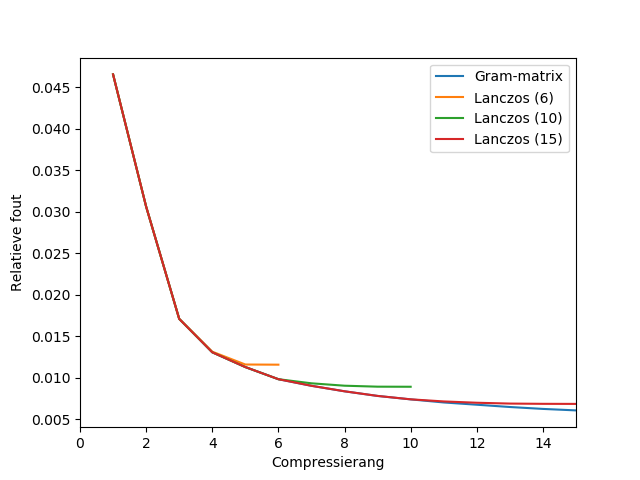
\includegraphics[scale=0.8]{images/lanczos_rank_comparison.png}
  \caption{Relatieve fout voor verschillende compressierangen en methoden bij het comprimeren van de eerste mode (de spectrale mode) van Cuprite. De getallen in de legende geven aan hoeveel Lanczos-iteraties uitgevoerd werden. Men ziet dat het nuttig kan zijn om meer iteraties uit te voeren dan de uiteindelijke compressierang.}
\label{fig:lanczos-rank-comparison}
\end{figure}

\subsubsection{Randomized SVD}

Wanneer we een afgeknotte SVD zoeken van een matrix $A \in \mathbb{R}^{m \times n}$ met $m \ll n$, zijn we eigenlijk ge\"interesseerd in de belangrijkste linker-singuliere vectoren, of met andere woorden, de beste basisvectoren om de verzameling kolomvectoren van $A$ in voor te stellen. Het is echter logisch dat vaak slechts een kleine deelverzameling van de kolomvectoren van $A$ al representatief is voor de volledige populatie en tot een even goede basis leidt. Op deze manier kan men de rekentijd van de SVD verkleinen zonder een grote fout te introduceren. Deze techniek wordt de \textit{randomized SVD} \cite{ref:randomized_svd} genoemd en wordt voor veel toepassingen gebruikt om de SVD te versnellen.\\

Concreet construeren we bij deze methode dus een matrix met een willekeurige verzameling kolommen van $A$ en berekenen we van deze steekproefmatrix de SVD om zo (de eerste kolommen van) $U$ te benaderen. De $\Sigma$ die hierbij berekend wordt is weliswaar niet accuraat, aangezien deze slechts het aandeel van de singuliere vectoren in de steekproef voorstelt, maar dit kan makkelijk gecorrigeerd worden door deze te vermenigvuldigen met $\sqrt{\frac{\text{populatiegrootte}}{\text{steekproefgrootte}}}$. Hierdoor wordt $\Sigma$ ook goed benaderd en kan deze gebruikt worden om bijvoorbeeld de compressierang te bepalen.\\

Verder kan de de SVD van de steekproefmatrix ook berekend worden met de bovenstaande methoden, om zo een grotere versnelling te bekomen.\\

\begin{table}[]
\centering
\begin{tabular}{|l|l|l|}
\hline
Methode & Gram-matrix & Steekproef + Gram-matrix\\ \hhline{|=|=|=|}
\input{data/randomized-svd-cuprite-test.tex}
\end{tabular}
\caption{Vergelijking tussen een typische uitvoering van de methode met de Gram-matrix met en zonder steekproef voor Cuprite met relatieve doelfout 0.025.}
\label{table:randomized-svd-cuprite-test}
\end{table}

In tabel \ref{table:randomized-svd-cuprite-test} vindt men een typische uitvoering met en zonder steekproef. Als steekproefgrootte per mode nemen we simpelweg 5 keer de originele rang. Merk op dat dit over slechts \'e\'en experiment gaat en men dus best geen conclusies trekt over bijvoorbeeld de absolute uitvoeringstijd. Wel kan men zien dat onze benaderingsmethode voor $\Sigma$ adequate precisie geeft. Verder geeft het gebruik van een steekproef in mode 2 een significante versnelling, terwijl in de andere modes de populatie te klein was ten opzichte van de originele rang om een steekproef te nemen. Uiteindelijk is er geen significante fout ge\"introduceerd door het gebruik van de steekproef.\\

\begin{table}[]
\centering
\begin{tabular}{|l|l|l|}
\hline
Methode & Gram-matrix & Steekproef + Gram-matrix\\ \hline
\input{data/randomized-svd-cuprite-average.tex}
\end{tabular}
\caption{Vergelijking tussen de methode met de Gram-matrix met en zonder steekproef voor Cuprite met relatieve doelfout 0.025 (10 experimenten).}
\label{table:randomized-svd-cuprite-average}
\end{table}

\begin{table}[]
\centering
\begin{tabular}{|l|l|l|}
\hline
Methode & Gram-matrix & Steekproef + Gram-matrix\\ \hline
\input{data/randomized-svd-mauna-kea-average.tex}
\end{tabular}
\caption{Vergelijking tussen de methode met de Gram-matrix met en zonder steekproef voor Mauna Kea met relatieve doelfout 0.025 (10 experimenten).}
\label{table:randomized-svd-mauna-kea-average}
\end{table}

We zien in tabel \ref{table:randomized-svd-cuprite-average} dat, voor deze dataset, de randomized SVD een degelijke versnelling geeft zonder een significant verschil in de fout of compressiefactor. Daarnaast is de variantie op de fout en compressiefactor erg klein. Bovendien toont tabel \ref{table:randomized-svd-mauna-kea-average} aan dat deze techniek ook goed werkt voor voor Mauna Kea, al is het met een steekproef van 20 keer de originele rang.\\

Verder hebben we als kleine optimizatie getest of het sorteren van de steekproefindices voor het selecteren van deze kolommen uit de steekproefmatrix effect heeft op de uitvoeringstijd. Dit kost rekenwerk maar kan eventueel een versnelling geven bij het kopi\"eren van de kolommen vanwege het betere \textit{memory access pattern}. In de praktijk bleef de rekentijd ongeveer hetzelfde, dus we gebruiken deze techniek verder niet.\\

\begin{figure}[]
  \centering
  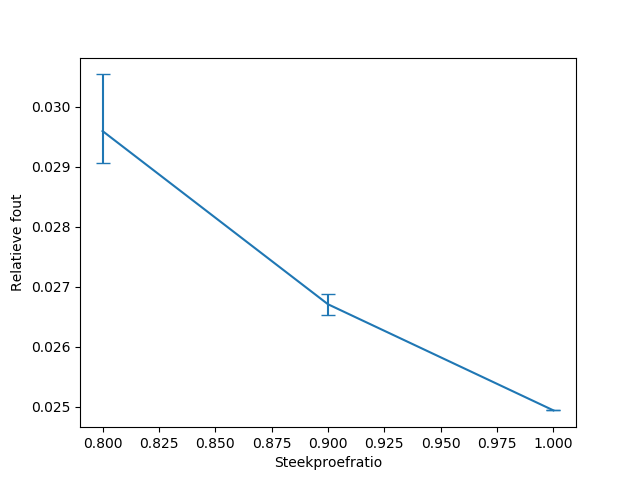
\includegraphics[scale=0.8]{images/randomized_svd_pavia_ratios.png}
  \caption{Compressiefout bij verschillende steekproefratios voor Pavia Centra met relatieve doelfout 0.025 (uitgemiddeld over 3 experimenten). De foutbalkjes stellen de minimale en maximale waarden voor over de verschillende experimenten.}
\label{fig:randomized-svd-pavia-ratios}
\end{figure}

In figuur \ref{fig:randomized-svd-pavia-ratios} ziet men echter dat de randomized SVD geen goede resultaten geeft bij Pavia Centre. Hierbij moesten we de steekproefratio (de verhouding tussen de steekproefgrootte en populatiegrootte) verhogen tot 1 om geen merkbare fout toe te voegen, maar in tabel \ref{table:randomized-svd-pavia-test} zien we dat een steekproefratio van 0.2 nog redelijk lijkt te werken voor de spectrale mode, de best comprimeerbare mode. Daarnaast zijn alle modes van Pavia significant slechter comprimeerbaar dan die van Cuprite. Hierdoor denken we dat de steekproefgrootte best groter gekozen wordt wanneer de mode slecht comprimeerbaar is.\\

De meest logische manier om de ``comprimeerbaarheid'' van een mode in te schatten, is echter door te kijken naar de verdeling van de singuliere waarden, die men pas kent na het berekenen van de SVD. Het lijkt ons dus moeilijk om voor een brede verzameling datasets op consistente wijze snel een goede steekproefgrootte te kiezen zonder verdere gegevens over de data, hoewel dit mogelijk verder onderzocht kan worden. Om deze reden zullen we de randomized SVD verder niet gebruiken, hoewel ze voor bepaalde datasets zeker een mooie versnelling kan opleveren.

\subsubsection{Besluit}

Na de resultaten van alle bovenstaande methodes te vergelijken, kiezen we ervoor om vanaf nu de methode met de Gram-matrix zonder verdere toevoegingen te gebruiken voor het berekenen van de SVD. Dit lijkt ons de snelste methode die geen significant effect heeft op de compressiefout- of factor.

\begin{table}[H]
\centering
\begin{tabular}{|l|l|l|}
\hline
Methode & Gram-matrix & Steekproef + Gram-matrix\\ \hhline{|=|=|=|}
\input{data/randomized-svd-pavia-test.tex}
\end{tabular}
\caption{Vergelijking tussen een uitvoering van de methode met de Gram-matrix met en zonder steekproef voor Pavia Centre met relatieve doelfout 0.025.}
\label{table:randomized-svd-pavia-test}
\end{table}
\section{Orthogonaliteitscompressie}

Men zou kunnen denken dat bij de Tuckerdecompositie de meeste ruimte ingenomen wordt door de kerntensor. Wanneer men namelijk naar tensoren met $k$ modes kijkt, waarbij de lengte per mode $n$ constant blijft en telkens gecomprimeerd wordt naar constante rang $r$, dan groeit de gecomprimeerde kerntensor met $O(r^k)$ en de factormatrices slechts met $O(knr)$, dus met $n, r$ constant en groeiende $k$ worden de factormatrices verwaarloosbaar.\\

In de praktijk werken we echter met een beperkt aantal modes en vaak lage compressierangen. Zelfs als we later reshapen verhogen we hiermeee $k$, maar verlagen we $n$ en $r$, dus het aandeel van de kerntensor zal hierdoor niet zozeer veel verhogen. Bijvoorbeeld, wanneer men de ST-HOSVD toepast op Cuprite met relatieve doelfout 0.025, comprimeert men van rang (512, 614, 190) naar (139, 192, 4) en nemen de factormatrices 64\% van het geheugen in. Bij Mauna Kea, een veel grotere dataset, is dit percentage 55\%. We kunnen dus concluderen dat het zeker interessant is om te kijken naar specifieke compressietechnieken voor de factormatrices.\\

We weten dat de factormatrices orthogonaal zijn en dit kunnen we benutten. Stel namelijk, we hebben een factormatrix $U \in \mathbb{R}^{n \times r}$ en verdelen deze op de volgende wijze:
\[
U = \begin{bmatrix}
A & c & \dots \\
B & x & \dots \\
\end{bmatrix}
\]
met $A \in \mathbb{R}^{(n-k) \times k}$, $B \in \mathbb{R}^{k \times k}$, $c \in \mathbb{R}^{n-k}$, $x \in \mathbb{R}^{k}$, voor willekeurige $1 \leq k < n$. Vanwege orthogonaliteit weten we dat:
\begin{align*}
\begin{bmatrix}
A \\
B \\
\end{bmatrix}^T
\begin{bmatrix}
c \\
x \\
\end{bmatrix}
&= 0 \\
A^T c + B^T x &= 0 \\
B^T x &= -A^T c
\end{align*}
Bijgevolg kunnen we $x$ berekenen als de oplossing van een lineair stelsel met $k$ onafhankelijke vergelijkingen en $k$ variabelen en moeten deze waarden niet opgeslagen worden. Theoretisch gezien kan men dus, door dit proces sequentieel uit te voeren voor $k = 1, \dots, n - 1$, een hele driehoek van $r (r - 1)/2$ elementen uit de matrix laten vallen. Om terug te komen op de eerdere voorbeelden: dit zou bij Cuprite en Mauna Kea neerkomen op 9.4\% en 7.5\% van alle waarden (inclusief kerntensor) respectievelijk. Men kan ook kiezen om de kolommen in een andere volgorde te verwerken, maar dit leek ons het beste zodat de herberekende waarden vooral zitten in de latere singuliere vectoren, die minder belangrijk zijn.
\section{Quantisatie}
\label{sec:quantisatie}

Tot nu toe hebben we altijd gewerkt met 32-bit floating-point getallen, wat voor onze doeleinden genoeg rekenprecisie geeft. Wanneer we deze getallen echter willen opslaan, zouden we ze liefst compacter willen voorstellen. Dit gaan we doen door te quantiseren: hierbij ronden we elke waarde af naar de dichtsbijzijnde waarde uit een beperkte verzameling die we zelf defini\"eren. Deze afronding zal de uiteindelijke fout op het eindresultaat verhogen, maar door deze verzamelingen goed te kiezen zullen we proberen een optimale afweging tussen de compressiefout en -factor te bekomen.\\

Wanneer we in deze sectie spreken over ``quantiseren naar $b$ bits'', doen we dit door de originele waarden te verschuiven en te schalen met specifieke waarden (die mee opgeslagen worden als 32-bit floats), zodat het nieuwe bereik exact overeenkomt met $[0, 2^b - 1]$. Hierna bekomen we de gequantiseerde waarden door alle waarden af te ronden naar het dichtsbijzijnde gehele getal. Dit is niet de enige mogelijke transformatie, maar we zullen ons in deze tekst hiertoe beperken. Verder zullen we de compressiefactor meten door telkens te quantiseren naar een verzameling met grootte gelijk aan $2^b$ (niet zozeer altijd met dezelfde $b$), waarna de geheugenruimte van per waarde geteld wordt als $b$ bits. 

\subsection{Kerntensor}

We zullen pas in de volgende subsectie quantisatietechnieken voor de factormatrices bespreken, maar zullen toch voor de komende experimenten moeten kiezen hoe deze verwerkt worden om de fout op het eindresultaat te berekenen. Zoals we in de vorige sectie zagen, wordt er quasi geen fout toegevoegd door de factormatrices te quantiseren naar 16 bits (en $\tau$ niet te quantiseren), dus we zullen dit ook doen voor de rest van de deze subsectie.

\subsubsection{Structuur van de kerntensor}

We weten dat gedurende de ST-HOSVD, bij het berekenen van de co\"ordinaten in de nieuwe basis, de eerste basisvectoren belangrijker zijn. Hierdoor zullen de absolute waarden van de eerste co\"ordinaten typisch ook groter zijn. Door dit proces meerdere malen toe te passen terwijl men over de modes itereert, zal men in feite de ``energie'' van de tensor concentreren in de posities met lage indices. De waarden in de uiteindelijke kerntensor zullen dus niet uniform verdeeld zijn.\\

Om hiermee rekening te houden zullen we in de rest van deze subsectie werken met ``lagen''. Met laag $i$ van een tensor bedoelen we de verzameling van posities met alle indices kleiner dan of gelijk aan $i$ en minstens \'e\'en index gelijk aan $i$ (denk aan schillen). In figuur \ref{fig:core-tensor-layers} wordt dit ge\"illustreerd. In de praktijk is de ongelijkheid tussen de lagen erg groot (zie figuur \ref{fig:core-tensor-values-distribution}, let op de logaritmische schaal).\\

\begin{figure}[H]
  \centering
  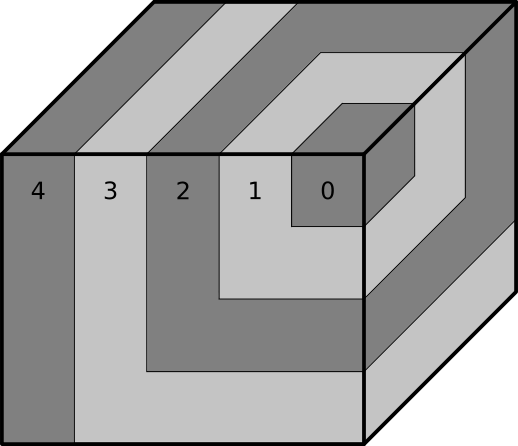
\includegraphics[scale=0.7]{images/core_tensor_layers.png}
  \caption{Lagen 0, \dots, 4 in een $5 \times 4 \times 3$ tensor.}
\label{fig:core-tensor-layers}
\end{figure}
\begin{figure}[H]
  \centering
  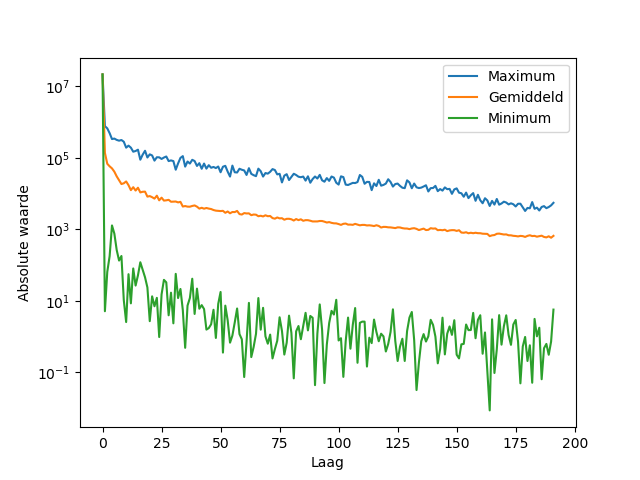
\includegraphics[scale=0.7]{images/core_tensor_values_distribution.png}
  \caption{Verdeling van absolute waarden in kerntensor bij Cuprite met relatieve doelfout 0.025.}
\label{fig:core-tensor-values-distribution}
\end{figure}

\newpage
Aangezien de meeste informatie in de eerste lagen zit, zullen we deze ongequantiseerd opslaan als 32-bit floats. Figuur \ref{fig:core-tensor-unquantized-portion} toont het effect van het aantal ongequantiseerde lagen bij vari\"erende aantallen quantisatiebits. Als quantisatietechniek gebruiken we simpelweg globale quantisatie: alle waarden buiten de eerste lagen worden gequantiseerd met hetzelfde aantal bits. Men ziet dat al een klein aantal lagen niet quantiseren een groot effect heeft op de fout met een insignificant effect op de compressiefactor. We kiezen ervoor om in het algemeen het aantal ongequantiseerde lagen zo te kiezen dat de norm van deze waarden minstens gelijk is aan 99.5\% van de norm van de tensor, wat bij Cuprite met relatieve doelfout 0.025 neerkomt op slechts 2 lagen.

\begin{figure}[H]
  \centering
  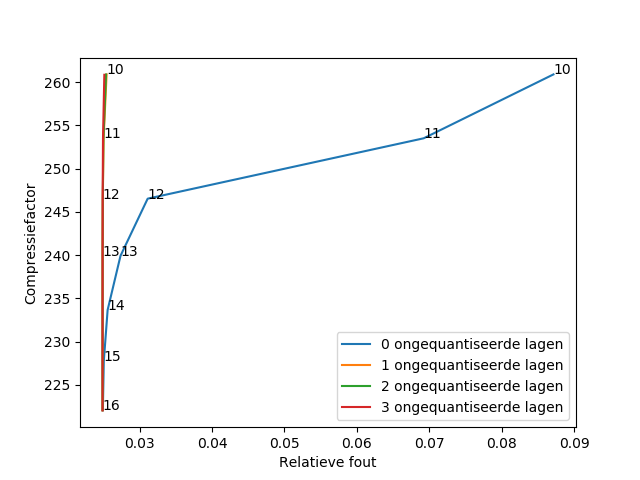
\includegraphics[scale=0.7]{images/core_tensor_unquantized_portion.png}
  \caption{Relatieve fout versus compressiefactor bij Cuprite met relatieve doelfout 0.025. De labels geven het aantal quantisatiebits aan.}
\label{fig:core-tensor-unquantized-portion}
\end{figure}

\subsubsection{Gelaagde quantisatie met constant aantal bits}

Zoals we eerder in figuur \ref{fig:core-tensor-values-distribution} zagen, zijn de waarden binnen de kerntensor erg ongelijk verdeeld, zelfs na het wegfilteren van de eerste twee lagen. Het is dus erg verspillend om alle andere waarden te quantiseren met hetzelfde aantal bits en dezelfde quantisatiestap, want het bereik van de waarden zal gedomineerd worden door het bereik van de eerste lagen, terwijl de laatste lagen slechts een erg klein deel van dit spectrum gebruiken.\\

Om dit op te lossen kunnen we elke laag apart quantiseren met een vast aantal bits dat constant blijft over de hele tensor, waardoor het bereik mooi past voor elke laag. Hierbij moeten we wel metadata gaan opslaan per laag en aangezien deze groeit met de afmetingen van de tensor zullen we deze meetellen in het geheugengebruik. Echter, bij een effici\"ente implementatie komt dit slechts neer op 12 bytes per laag, dus de \textit{overhead} van deze techniek is erg beperkt.

\subsubsection{Gelaagde quantisatie met variabel aantal bits}

Door het aantal quantisatiebits constant te houden over verschillende lagen, zal de quantisatiestap fijner worden voor de latere lagen. We weten echter dat alle kolommen uit de factormatrices genormaliseerd zijn, dus een vaste absolute fout op een waarde in de kerntensor zal zich onafhankelijk van de positie van deze waarde vertalen naar ongeveer dezelfde fout op het eindresultaat. Het is dus logischer om de latere lagen te quantiseren met een even grote stap, waardoor we minder bits nodig hebben.\\

Bij deze techniek zullen we voor elke laag een nieuw aantal quantisatiebits kiezen. We minimaliseren dit aantal zodat de quantisatiestap voor deze laag onder een bepaalde maximale stapgrootte ligt. We zullen deze controleren door expliciet het aantal quantisatiebits voor de eerste ongequantiseerde laag (de bits-parameter) te kiezen en dan de resulterende quantisatiestap gebruiken als bovengrens voor de verdere lagen. Voor het opslaan van het gekozen aantal bits zullen we \'e\'en byte extra per laag tellen, maar dit heeft natuurlijk geen significant effect.

\begin{figure}[H]
  \centering
  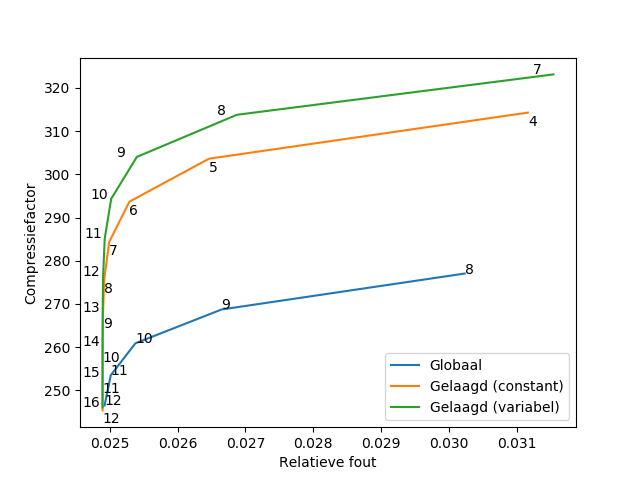
\includegraphics[scale=0.7]{images/core_tensor_quantization_comparison.png}
  \caption{Relatieve fout versus compressiefactor bij Cuprite met relatieve doelfout 0.025 en verschillende quantisatiemethoden voor de kerntensor. De labels geven de bits-parameterwaarden aan.}
\label{fig:core-tensor-quantization-comparison}
\end{figure}

\subsubsection{Besluit}

We hebben drie mogelijke quantisatietechnieken voor de kerntensor besproken: globale quantisatie en gelaagde quantisatie met een constant of variabel aantal bits. In figuur \ref{fig:core-tensor-quantization-comparison} zien we een experimentele vergelijking. Zoals verwacht comprimeert globale quantisatie het slechtste en kan men de gelaagde quantisatie verbeteren door te werken met een variabel aantal bits. Omwille van dit resultaat zullen we vanaf nu deze laatste techniek gebruiken (en specifiek voor de rest van deze sectie en sectie \ref{sec:encodering} met een bits-parameter van 12).

\subsection{Factormatrices}
\label{sec:quantisatie-factor-matrices}

Na de orthogonaliteitscompressie zal elke factormatrix voorgesteld worden als de combinatie van reflectoren en $\tau$-waarden (die samengevoegd worden tot \'e\'en $\tau$-vector per factormatrix). Zoals eerder besproken zullen we de $\tau$-vectoren niet quantiseren, omdat deze belangrijker zijn dan de andere waarden in de factormatrices en ons slechts 4 bytes per kolom per factormatrix kost. De waarden van de reflectoren nemen echter veel ruimte in en moeten best gequantiseerd worden.

\begin{figure}[H]
  \centering
  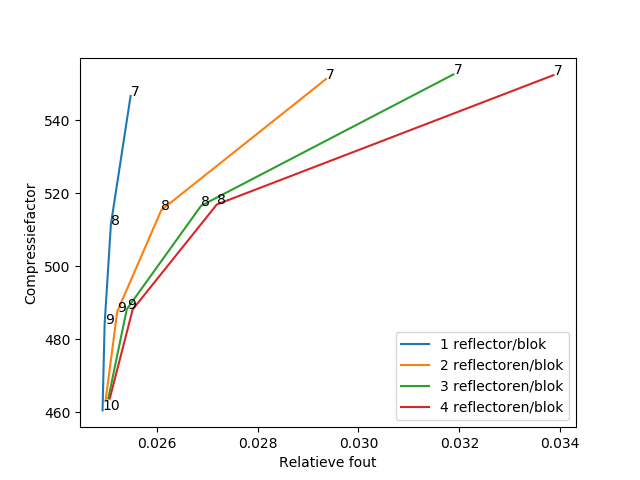
\includegraphics[scale=0.7]{images/factor_matrix_quantization_block_cols.png}
  \caption{Relatieve fout versus compressiefactor bij Cuprite met relatieve doelfout 0.025 en verschillende blokgroottes voor de quantisatie van de factormatrices. Quantisatie gebeurde gelaagd met norm-gebaseerde bit-aantal-selectie (zie vervolg subsectie). De labels geven de bits-parameterwaarden aan.}
\label{fig:factor-matrix-quantization-block-cols}
\end{figure}

Een eerste manier om dit te doen is weer met globale quantisatie per factormatrix (dus we berekenen \'e\'en specifiek bereik per matrix, niet voor alle matrices samen). We zagen echter al in de vorige subsectie dat het nuttig is om de waarden onder te verdelen in blokken, waardoor een specifieker bereik kan worden vastgelegd. Een gemiddelde reflector uit een factormatrix bevat echter veel minder waarden dan een gemiddelde laag uit de kerntensor, dus men zou kunnen proberen om meerdere reflectoren te groeperen per blok om zo de \textit{overhead} van de metadata (12 bytes per blok, eventueel 1 byte extra bij een variabel aantal bits) te beperken. Desalniettemin toont figuur \ref{fig:factor-matrix-quantization-block-cols} aan dat het beter is om dit niet te doen. We hebben ook ge\"experimenteerd met technieken om het aantal reflectoren per blok dynamisch te kiezen in functie van de dimensie van de reflector en het aantal quantisatiebits, maar dit gaf hetzelfde resultaat.\\

Om het aantal quantisatiebits te selecteren, kunnen we ook verschillende methoden gebruiken. De simpelste optie is om de bits-parameter te gebruiken als het constante aantal quantisatiebits voor elke reflector, maar hierbij houdt men geen rekening met enkele aspecten:

\begin{enumerate}

\item De eerste reflector be\"invloedt de reconstructie van alle kolommen van de factormatrix, de tweede reflector be\"invloedt alle kolommen buiten de eerste, ... Bijgevolg zijn de eerste reflectoren belangrijker en zou men deze met meer precisie kunnen bijhouden. Aangezien dit effect moeilijk te quantiseren valt houden we hier geen rekening mee.

\item De eerste singuliere vectoren zijn belangrijker dan de laatste, waardoor we beter meer precisie gebruiken voor deze. Bij ``norm-gebaseerde'' selectie zullen we het aantal bits per waarde binnen een reflector ongeveer proportioneel kiezen met het logaritme van de norm van de corresponderende snede uit de kerntensor (de waarden die later vermenigvuldigd zullen worden met corresponderende singuliere vector). De bits-parameter legt vast hoeveel quantisatiebits er voor de eerste reflector gekozen moeten worden.

\item De eerste reflectoren hebben een hogere dimensie en worden dus voorgesteld door meer waarden, waardoor het aantal bits per waarde hier misschien verlaagd moet worden. Bij ``norm- en dimensie-gebaseerde'' selectie zal het totaal aantal gebruikte bits per reflector ongeveer proportioneel zijn met de norm van de corresponderende snede uit de kerntensor. Zoals eerder wordt het aantal quantisatiebits per waarde voor de eerste reflector vastgelegd door de bits-parameter.

\end{enumerate}

In figuur \ref{fig:factor-matrix-quantization-comparison} vindt men een vergelijking van de besproken methoden. Zoals verwacht is gelaagde quantisatie opnieuw veel beter. Voor de bitselectie is de norm-gebaseerde techniek het beste, gevolgd door de norm- en dimensie-gebaseerde techniek en uiteindelijk constante selectie. Men zou dit kunnen verklaren door het effect van het eerste aspect dat we eerder bespraken (omzetting van reflectoren naar singuliere vectoren). Dit hebben we namelijk niet in rekening gebracht maar zou de norm-gebaseerde selectie moeten helpen. In ieder geval is dit de beste techniek en zal deze vanaf nu gebruikt worden. Voor de volgende sectie zullen we werken met een bits-parameter van 10, waardoor er geen merkbare fout toegevoegd zal worden.

\begin{figure}[H]
  \centering
  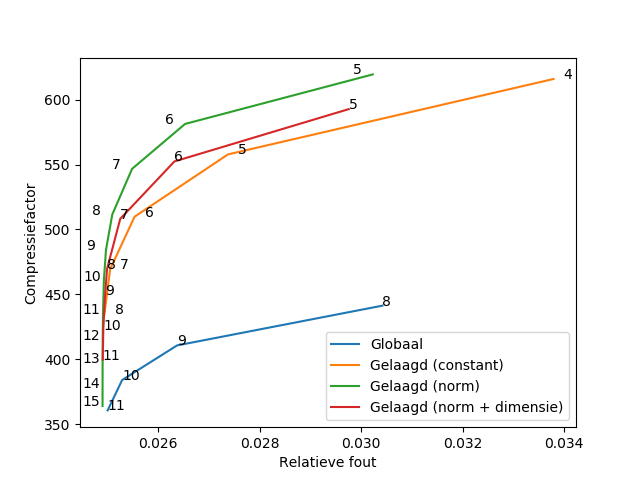
\includegraphics[scale=0.6]{images/factor_matrix_quantization_comparison.png}
  \caption{Relatieve fout versus compressiefactor bij Cuprite met relatieve doelfout 0.025. De labels geven de bits-parameterwaarden aan.}
\label{fig:factor-matrix-quantization-comparison}
\end{figure}
\section{Encodering en lossless compressie}
\label{sec:encodering}

Nadat we de waarden van de kerntensor en factormatrices gequantiseerd hebben, encoderen we deze naar bits, voegen we deze samen in \'e\'en lange bitstring en comprimeren deze met Deflate om de finale compressie te bekomen. We bespreken in deze sectie enkele keuzes die nog gemaakt moeten worden bij de encodering, gevolgd door een kort deel over de effici\"entie van de implementatie.

\subsection{Encoderingsmethoden}

Er zijn verschillende manieren om gehele getallen uit $\{0, \dots, 2^b - 1\}$ om te zetten naar een bitstring:
\begin{itemize}

\item \textbf{Standaard:} We schrijven het getal in binair, met de meest significante bit eerst.

\item \textbf{Gray-code \cite{ref:graycode}:} Zoals de standaard-encodering, encoderen Gray-codes waarden uit $\{0, \dots, 2^b - 1\}$ elk naar een codewoord van constante lengte ($b$ bits), maar met de eigenschap dat de encodering van twee opeenvolgende getallen altijd verschilt in juist \'e\'en bit. Dit betekent dat, als de meeste waarden geconcentreerd zijn rond een bepaald punt, dat een groot deel van de bits in de encodering van elke waarde nog gelijk zullen zijn. Dit zou eventueel beter gecomprimeerd kunnen worden door Deflate.

\item \textbf{Huffman-code \cite{ref:huffman_coding}:} Bij Huffman-encodering worden de verschillende symbolen voorgesteld door codewoorden van variabele lengte, zodat veel voorkomende symbolen ge\"encodeerd worden als korte codewoorden. Dit is erg effici\"ent als men de prefix-boom al kent. In ons geval zullen we echter voor elke quantisatieblok de optimale code berekenen en de bijhorende boom opslaan in een simpel binair formaat (gebaseerd op een post van Stack Overflow \cite{ref:huffman_tree}). In dit formaat neemt de boom $(b + 2)*n - 1$ bits in, voor een verzameling van $n$ unieke symbolen, elk initieel voorgesteld door $b$ bits (we zullen de bomen ook nog comprimeren met Deflate om de opslag te minimaliseren). Voor grote quantisatieblokken met veel herhalende symbolen is dit dus niet zo groot meer.

\item \textbf{Adaptief:} Voor kleine blokken kan deze \textit{overhead} veroorzaakt door de opslag van de bomen echter een probleem vormen. Om deze reden ontwikkelden we ook een adaptieve methode: voor elke quantisatieblok wordt gekozen uit een Gray-code, benaderende Huffman-code (zie verder) of exacte Huffman-code, op basis van het kleinste geheugengebruik (inclusief de opslag van de boom). Het opstellen en vergelijken van deze verschillende codes voor elke blok kost echter een significante hoeveelheid tijd (zelfs met een optimalisatie waarbij de exacte Huffman-code niet berekend wordt als men op voorhand al ziet dat de boom te groot gaan zijn).\\

\begin{figure}[H]
\centering
\begin{subfigure}{0.44\textwidth}
  \centering
  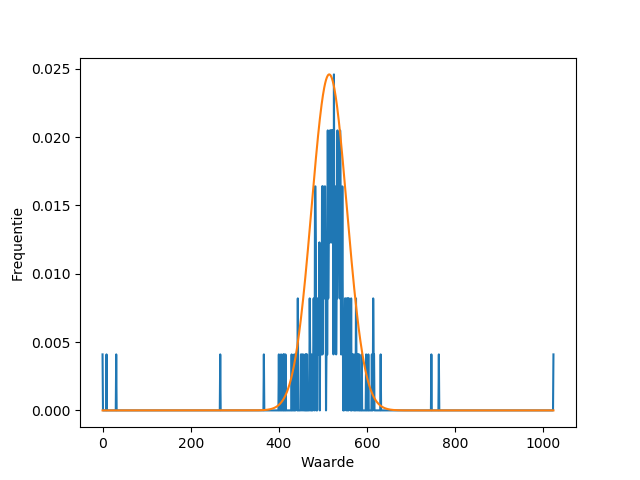
\includegraphics[width=0.9\linewidth]{images/distribution_quantized_values_layer_30.png}
  \caption{Laag 30}
\end{subfigure}
\begin{subfigure}{.44\textwidth}
  \centering
  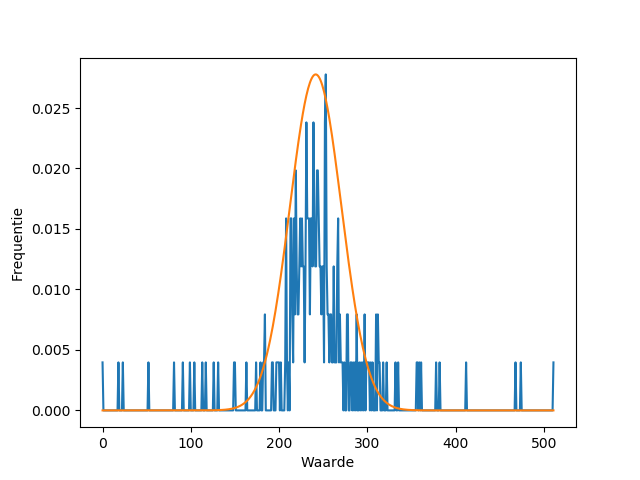
\includegraphics[width=0.9\linewidth]{images/distribution_quantized_values_layer_31.png}
  \caption{Laag 31}
\end{subfigure}
\\
\begin{subfigure}{.44\textwidth}
  \centering
  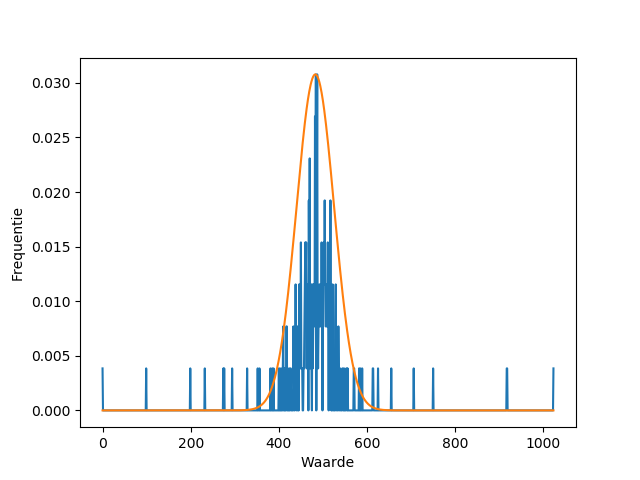
\includegraphics[width=0.9\linewidth]{images/distribution_quantized_values_layer_32.png}
  \caption{Laag 32}
\end{subfigure}
\begin{subfigure}{.44\textwidth}
  \centering
  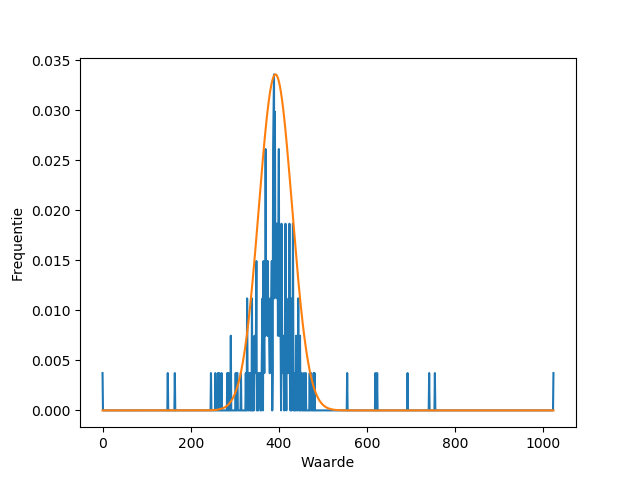
\includegraphics[width=0.9\linewidth]{images/distribution_quantized_values_layer_33.png}
  \caption{Laag 33}
\end{subfigure}
\caption{Verdeling van gequantiseerde waarden binnen een quantisatieblok. Elke grafiek is een voorbeeldblok uit de kerntensor van Cuprite bij relatieve doelfout 0.025. De blauwe lijnen zijn de echte voorkomens (frequenties) van de waarden, de oranje lijnen zijn de Gaussische benaderingen.}
\label{fig:distribution-quantized-values}
\end{figure}

Als men kijkt naar figuur \ref{fig:distribution-quantized-values} ziet men dat voor middelmatig grote quantisatieblokken, er al wat structuur ontstaat in de verdeling van de waarden. Hoewel er nog niet genoeg waarden zijn om een volledige Huffman-boom voor op te slaan, is het gebruik van een standaard encodering of Gray-codes ook niet optimaal.\\

In plaats hiervan introduceren we een nieuwe techniek: een benaderende Huffman-code (BHC). Hierbij berekenen we de Huffman-code, niet met de frequenties van de symbolen in de originele data, maar met de functiewaarden van een Gaussische benadering van deze frequenties. Dit leidt nog steeds tot een redelijk effici\"ente encodering (zie figuur \ref{fig:distribution-quantized-values} voor de nauwkeurigheid van de benadering), want veel voorkomende symbolen zullen door kortere codes voorgesteld worden. De code zelf wordt echter volledig vastgelegd door twee 32-bit floats die de Gaussische benadering defini\"eren ($\mu$ en $\sigma$) en kan dus in slechts 8 bytes opgeslagen worden.\\

In de praktijk betekent dit wel dat men een compleet deterministisch algoritme moet schrijven om de boom te construeren op basis van deze $\mu$ en $\sigma$. Dit zijn echter geen gehele getallen, dus het is niet triviaal om code te schrijven die zelfs na veranderingen in hardware en software nog steeds altijd dezelfde discrete beslissingen neemt op basis van floating-point rekenwerk. Dit lijkt ons mogelijk, maar wel een extra implementatie-uitdaging. In onze onderzoeksomgeving zullen we hier echter geen last van hebben, aangezien we de gecomprimeerde data meteen terug decomprimeren met dezelfde code, dezelfde hardware en dezelfde onderliggende software.

\end{itemize}

\subsection{Endianness}

Uiteindelijk zullen we de bitstring terug moeten omzetten naar een reeks bytes. Elke groep van 8 bits kan dan op twee manieren ge\"interpreteerd worden: met de minst (\textit{little-endian}) of meest (\textit{big-endian}) significante bits eerst. Deze keuze zou technisch gezien een klein effect kunnen hebben op hoe Deflate het resultaat interpreteert en comprimeert, dus we hebben deze beide getest.

\subsection{Implementatie}

We kozen ervoor om de encodering te implementeren met de Python-module \texttt{bitarray} \cite{ref:bitarray}. Aangezien deze in C is geschreven is dit veel sneller dan enige Python-routines die we zelf zouden maken. Toch ontbrak er effici\"ente ondersteuning voor twee zaken:

\begin{itemize}

\item De module ondersteunt prefix codes van variabele lengte \cite{ref:variable_length_code} door bij het encoderen/decoderen te vragen naar een \textit{map} van elk symbool naar diens binaire voorstelling. Elke keer wanneer we een quantisatieblok decoderen zal de module echter een boom moeten construeren om snel de bitstring te \textit{parsen}. Deze constructie duurt erg lang en is niet nodig voor codes van constante lengte (zoals de standaard-encodering of Gray-codes). We hebben een nieuwe iterator toegevoegd om te decoderen op basis van zo'n code, waardoor dit proces enorm versneld is.

\item Voor Huffman-codes \cite{ref:huffman_coding} kunnen we deze iterator dus niet gebruiken, want deze codes hebben een variabele lengte. Om dit op te lossen hebben we ook een functie toegevoegd om de prefix-boom door te geven als een bitstring in het formaat dat in de volgende subsectie besproken zal worden. Dit omzeilt de trage omzetting van \textit{map} naar boom en geeft ook een grote versnelling.

\end{itemize}

Verder werd er bij de implementatie van dit deel gebruik gemaakt van van verschillende stukken code van het internet. Aangezien het gaat over algemeen bekende technieken (zoals Gray-codes en Huffman-codes) en geen origineel onderzoek leek dit ons geen probleem. In ieder geval staan alle bronnen van gekopieerde code vermeld in de broncode in bijlage \ref{app:algoritmen}.

\subsection{Besluit}

In tabel \ref{table:encoding-comparison1} vindt men de uiteindelijke groottes van de gecomprimeerde uitvoer. Ten eerste merken we op dat \textit{endianness} geen significant effect heeft, dus we zullen deze vanaf nu altijd als \textit{big-endian} kiezen. Aangezien het comprimeren met Deflate vaak een kleine verbetering geeft, zullen we dit ook standaard doen in de toekomst.\\

\begin{table}[H]
\centering
\begin{tabular}{|l|c|c|c|c|}
\hline
& \multicolumn{2}{c|}{Geen Deflate} & \multicolumn{2}{c|}{Deflate} \\ \cline{1-5} 
\textit{Endianness} & Little & Big & Little & Big \\ \hline
\input{data/encoding-comparison1.tex}                             
\end{tabular}
\caption{Grootte van gecomprimeerde versies van Cuprite (in bytes) voor verschillende encoderingen voor en na compressie met Deflate. Parameters: relatieve doelfout 0.025, bits-parameter voor de kerntensor 12 en bits-parameter voor de factormatrices 10.}
\label{table:encoding-comparison1}
\end{table}

Wanneer we de verschillende encoderingsmethoden bekijken, zien we dat Huffman-encodering eigenlijk veel slechter is dan de standaard encodering of Gray-codes. De verklaring vindt men in tabel \ref{table:encoding-comparison2}: de data zelf wordt significant effici\"enter ge\"encodeerd, maar de bomen kosten te veel ruimte om op te slaan. Hierdoor is de adaptieve encoderingsmethode de beste keuze op vlak van compressiefactor: hierbij worden er alleen Huffman-bomen opgeslagen wanneer dit de totale opslagruimte verlaagt.

\newpage
\begin{table}[H]
\centering
\begin{tabular}{|l|c|c|c|}
\hline
Encoderingsmethode & Ge\"encodeerde data & Bomen & Totaal \\ \hline
\input{data/encoding-comparison2.tex}                             
\end{tabular}
\caption{Grootte van gecomprimeerde versies van Cuprite (in bytes).}
\label{table:encoding-comparison2}
\end{table}

In tabel \ref{table:encoding-timing} zien we echter dat de adaptieve methode veel trager is dan de alternatieven. Om dit aan te pakken zullen we vanaf nu werken met adaptieve encodering waarbij alleen gekozen wordt tussen Gray-codes en exacte Huffman-codes. Het kost namelijk relatief veel tijd om te werken met benaderende Huffman-codes. Op deze manier kunnen we de rekentijd verlagen met een factor 4 terwijl de compressiefactor verschilt met minder dan 0.5\%.

\begin{table}[H]
\centering
\begin{tabular}{|l|c|c|}
\hline
Encoderingsmethode & Relatieve grootte & Totale tijd (s) \\ \hline
\input{data/encoding-timing.tex}                             
\end{tabular}
\caption{Grootte (relatief ten opzichte van het minimum) van gecomprimeerde versies van Cuprite versus uitvoeringstijd voor verschillende encoderingsmethoden (10 experimenten). De totale tijd is hier gedefinieerd als de compressie- en decompressietijd van de quantisatie- en encoderingsfase.}
\label{table:encoding-timing}
\end{table}
\section{Afstellen van de parameters}

Na de beslissingen die gemaakt werden in de eerdere secties, blijven er drie parameters over die de compressiefactor en -fout van de uitvoer bepalen: de relatieve doelfout tijdens de ST-HOSVD (RDS), de bits-parameter voor de quantisatie van de kerntensor (BPK) en de bits-parameter voor de quantisatie van de factormatrices (BPF). Het is echter niet triviaal om deze drie optimaal te kiezen om bijvoorbeeld de compressiefactor te maximaliseren met bij een bepaalde compressiefout. In deze sectie zullen we proberen een algoritme te ontwerpen dat in beperkte rekentijd goede parameterwaarden kan bepalen.\\

Helaas duurt de compressie en decompressie van grote datasets te lang om met een groot aantal parameterwaarden te experimenteren, dus we zullen ons in onze analyse beperken tot twee kleinere gevallen: Cuprite en Indian Pines.

\subsection{Niet-adaptieve selectie}

Om een idee te krijgen van de optimale parameterwaarden voor een bepaalde relatieve fout, zullen we eerst een groot aantal experimenten uitvoeren met vari\"erende waarden. Hierbij gebruiken we de volgende domeinen:

\begin{itemize}
\item $RDS \in \{0.005, 0.075, 0.01, \dots, 0.05\}$
\item $BPK \in \{16, 15, 14, \dots, 1\}$
\item $BPF \in \{16, 15, 14, \dots, 1\}$
\end{itemize}

We kunnen aannemen dat (bijna altijd) het verhogen van de RDS, verlagen van de BPK of verlagen van de BPF de uiteindelijke compressiefout zal vergroten. Daarnaast zijn we vooral ge\"interesseerd in relatieve doelfouten kleiner dan 0.05. Bijgevolg zullen we, eens dat er een experiment een fout voorbij deze grens gaf, geen experimenten meer proberen met grotere (of gelijke) RDS en lagere (of gelijke) BPK en BPF, want deze geven sowieso een grotere fout. Op deze manier kunnen we de parameterruimte sneller doorzoeken.

\begin{figure}[H]
  \centering
  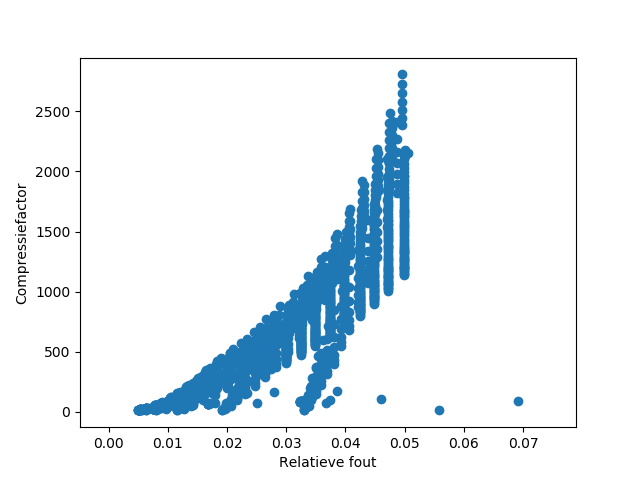
\includegraphics[scale=0.7]{images/all_sweep_points_cuprite.png}
  \caption{Resultaten voor vari\"erende parameters voor Cuprite. Elk punt stelt \'e\'en experiment voor, met een unieke combinatie van parameterwaarden.}
  \label{fig:all_sweep_points_cuprite}
\end{figure}

In figuur \ref{fig:all_sweep_points_cuprite} zien we de volledige verzameling uitgevoerde experimenten op \'e\'en grafiek (voor Cuprite). De meeste punten zijn echter niet interessant. Stel namelijk, elk experiment $E_i$ geeft een relatieve fout $RF_i$ en compressiefactor $CF_i$. Als men dan twee experimenten $E_i$ en $E_j$ beschouwt, met $RF_i < RF_j$ en $CF_i > CF_j$, dan is het resultaat van $E_i$ op beide vlakken beter en is $E_j$ zeker een suboptimaal resultaat. Na het wegfilteren van dergelijke suboptimale punten bekomen we de curve uit figuur \ref{fig:filtered_sweep_points_cuprite}. Vanaf nu zullen we dit de steekproefoptima noemen, aangezien deze nog steeds gelimiteerd zijn door de eerder gekozen domeinen voor de parameterwaarden. Vooral voor grote fouten begint deze beperking merkbaar te worden en wordt de curve minder continu.

\begin{figure}[H]
  \centering
  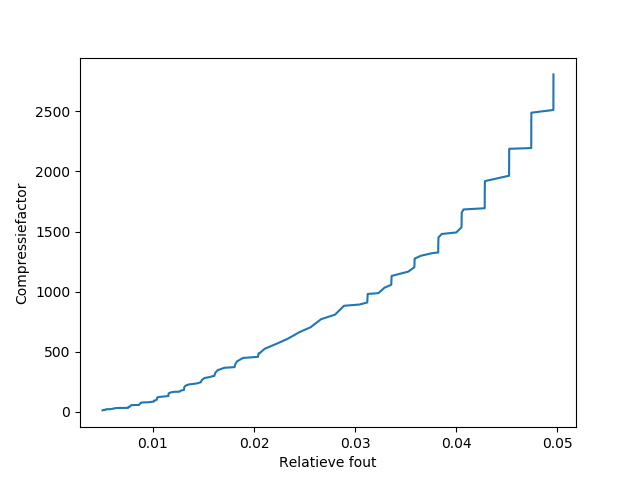
\includegraphics[scale=0.7]{images/filtered_sweep_points_cuprite.png}
  \caption{Resultaten voor vari\"erende parameters voor Cuprite, zonder suboptimale punten.}
  \label{fig:filtered_sweep_points_cuprite}
\end{figure}

In figuren \ref{fig:filtered_sweep_points_RDS}, \ref{fig:filtered_sweep_points_BPK} en \ref{fig:filtered_sweep_points_BPF} zien we welke parameterwaarden corresponderen met deze steekproefoptima. We voerden ook hetzelfde proces uit op Indian Pines. Voor elke parameter leggen we nu een selectiefunctie vast op basis van deze experimentele resultaten. Het kiezen van deze functies kan geavanceerder en is zeker een piste voor verder onderzoek.

\begin{itemize}
\item $RDS = max(0.001, 0.962601*\text{kwaliteit} - 0.000414)$, simpelweg op basis van lineaire regressie. De resultaten voor Cuprite en Indian Pines liggen hier vrij dichtbij elkaar.
\item $BPK = max(10, round(-445.117*\text{kwaliteit} + 16.795))$. Deze functie werd bepaald aan de hand van lineaire regressie op de eerste waarden van Cuprite, gevolgd door een harde ondergrens van 10. Dit is weliswaar te groot voor Indian Pines, maar zoals we eerder zagen kan de fout erg snel escaleren wanneer het aantal quantizatiebits te laag gekozen wordt, dus we zullen gaan voor eerder conservatieve waarden.
\newpage

\begin{figure}[H]
  \centering
  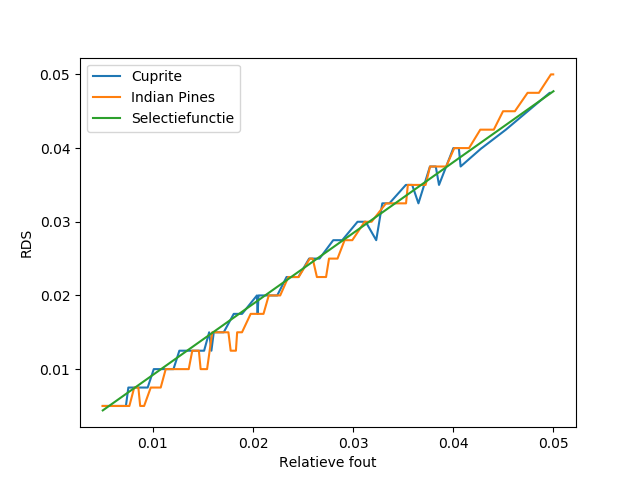
\includegraphics[scale=0.7]{images/filtered_sweep_points_RDS.png}
  \caption{RDS-waarden van steekproefoptima en de RDS-selectiefunctie.}
  \label{fig:filtered_sweep_points_RDS}
\end{figure}

\begin{figure}[H]
  \centering
  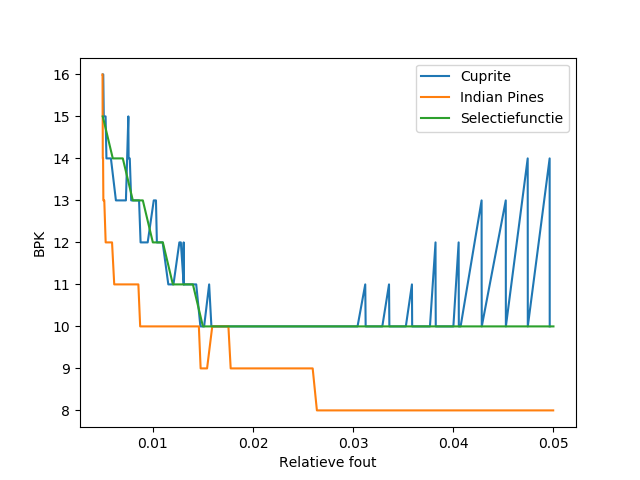
\includegraphics[scale=0.7]{images/filtered_sweep_points_BPK.png}
  \caption{BPK-waarden van steekproefoptima en de BPK-selectiefunctie. De grote sprongen bij de laatste waarden van Cuprite worden veroorzaakt door de beperkte selectie van RDS-waarden gedurende de experimenten.}
  \label{fig:filtered_sweep_points_BPK}
\end{figure}

\newpage

\begin{figure}[H]
  \centering
  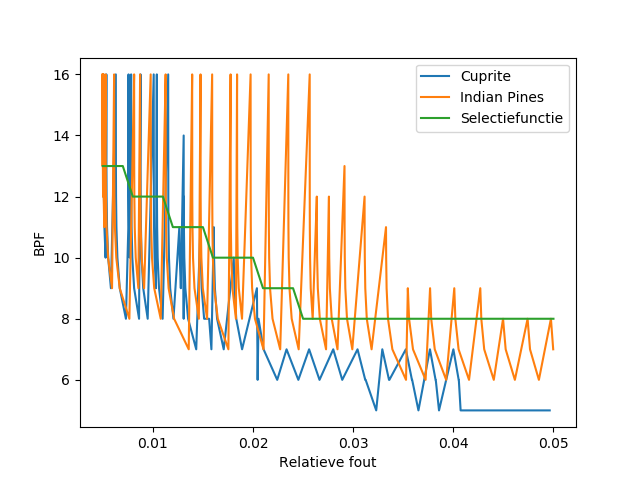
\includegraphics[scale=0.7]{images/filtered_sweep_points_BPF.png}
  \caption{BPF-waarden van steekproefoptima en de BPF-selectiefunctie.}
  \label{fig:filtered_sweep_points_BPF}
\end{figure}

\item $BPF = max(8, round(-228.571*quality + 14.143))$. We zien in de experimentele resultaten dat de exacte steekproefoptima sterk vari\"eren, dus we kozen ervoor om vooral naar het midden van de functies te kijken (we zullen zien dat dit geen plotselinge grote fouten geeft in onze eindresultaten, zie figuren \ref{fig:parameter_functions_results_Cuprite} en \ref{fig:parameter_functions_results_Indian_Pines}). Deze selectiefunctie werd gekozen op analoge wijze als de BPK-functie, maar deze keer net beperkt door resultaten van Indian Pines.
\end{itemize}

Met deze selectiefuncties hebben we compressies uitgevoerd waarbij de RDS, BPK en BPF automatisch bepaald werden op basis van \'e\'en enkele parameter, de kwaliteit. Als waarden voor de kwaliteitsparameter gebruikten we 0.005, 0.006, \dots, 0.05. De resultaten hiervan kan men vinden in figuren \ref{fig:parameter_functions_results_Cuprite} en \ref{fig:parameter_functions_results_Indian_Pines}. Voor kleine fouten lijken onze functies goed te werken, maar naarmate de fout stijgt verliezen we een deel van onze compressiefactor vanwege suboptimale parameterkeuzes.

\newpage
\begin{figure}[H]
  \centering
  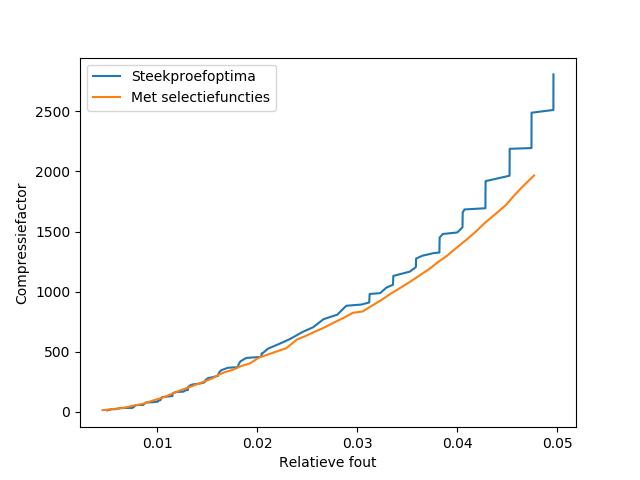
\includegraphics[scale=0.7]{images/parameter_functions_results_Cuprite.png}
  \caption{Resultaten van compressie met selectiefuncties voor Cuprite.}
  \label{fig:parameter_functions_results_Cuprite}
\end{figure}

\begin{figure}[H]
  \centering
  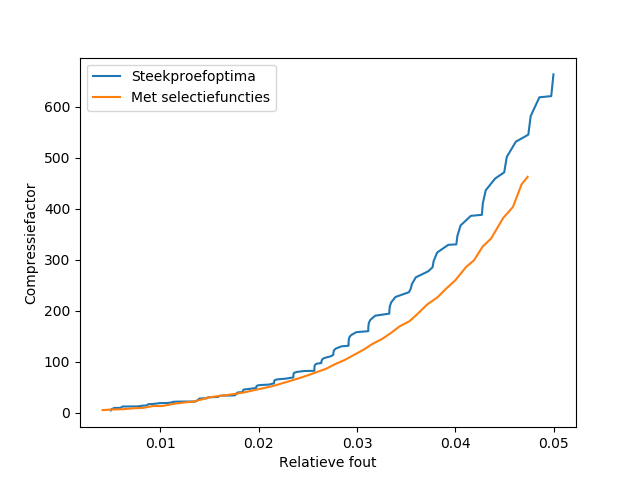
\includegraphics[scale=0.7]{images/parameter_functions_results_Indian_Pines.png}
  \caption{Resultaten van compressie met selectiefuncties voor Indian Pines.}
  \label{fig:parameter_functions_results_Indian_Pines}
\end{figure}

\newpage
\subsection{Adaptieve selectie}

Als we meer rekentijd mogen investeren, kunnen we echter betere parameters kiezen door gedurende de compressie simpelweg verschillende waarden uit te proberen en het beste resultaat te kiezen. Bij adaptieve selectie zullen we dit in beperkte mate proberen te doen.\\

Concreet maken we van de compressie een iteratief algoritme, waarbij we starten met dezelfde parameters als bij niet-adaptieve selectie. We zagen eerder dat de RDS-functie vrij onafhankelijk is van de dataset, waardoor we deze parameterwaarde niet meer zullen aanpassen. In elke iteratie testen we de uiteindelijke compressiefout en -factor zowel als men de BPK-waarde of de BPF-waarde met \'e\'en zou verlagen. Het algoritme kiest dan op basis van het huidige resultaat en de alternatieve resultaten welke parameter verlaagd wordt voor de volgende stap (de exacte beslissingsprocedure laten we hier buiten beschouwing). Als geen van beide verlaagd kan worden zonder dat de compressiefout de kwaliteitsparameter overschrijdt, stopt het algoritme.\\

Bij de implementatie werd weliswaar rekening gehouden met enkele optimisaties:
\begin{itemize}
\item Aangezien de RDS-waarde vast ligt, moet de ST-HOSVD en orthogonaliteitscompressie slechts \'e\'en keer uitgevoerd worden, zelfs met vari\"erende BPK en BPF.
\item Bij het berekenen van de alternatieve compressies, moet telkens maar de helft van de quantisatie- en encoderingsfasen uitgevoerd worden: alleen de kerntensor moet herberekend worden voor verlaagde BPK, alleen de factormatrices voor verlaagde BPF.
\item Elke iteratie moet slechts \'e\'en nieuw alternatief berekend worden, want het alternatief van de parameter die niet verlaagd werd kan hergebruikt worden. Het kost wel extra geheugen om deze compressies bij te houden.
\end{itemize}

In figuren \ref{fig:parameter_functions_results_including_adaptive_Cuprite} en \ref{fig:parameter_functions_results_including_adaptive_Indian_Pines} vindt men de experimentele resultaten van adaptieve parameterselectie. Men ziet dat men met deze techniek grote vooruitgang kan boeken op vlak van compressiefout en -factor. Door het beperkte domein van de RDS-waarden in de initi\"ele steekproef (waarmee we de optimale parameterwaarden probeerden te analyseren) verslaat adaptieve selectie zelfs de steekproefoptima.\\

In figuren \ref{fig:adaptive_timings_Cuprite} en \ref{fig:adaptive_timings_Indian_Pines} zien we echter dat adaptieve parameterselectie een significante kost heeft op vlak van compressietijd. Verder wordt er ook meer geheugen gebruikt voor het bijhouden van alternatieve compressies. Om deze redenen zullen we deze techniek in het algemeen proberen te gebruiken, tenzij de uitvoeringstijd naar ons oordeel onacceptabel is.

\newpage
\begin{figure}[H]
  \centering
  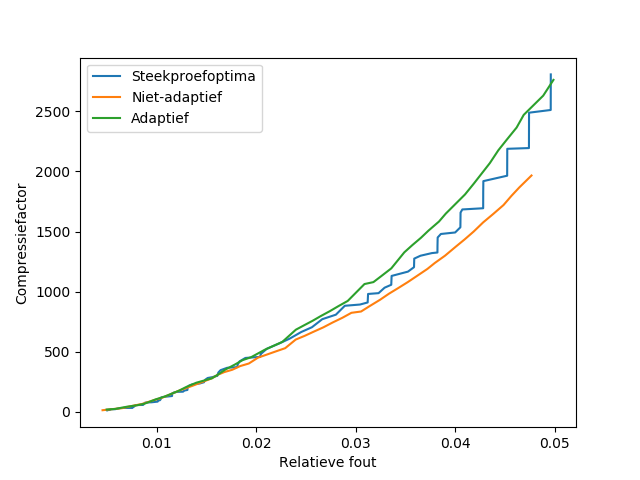
\includegraphics[scale=0.7]{images/parameter_functions_results_including_adaptive_Cuprite.png}
  \caption{Resultaten van compressie met adaptieve parameterselectie voor Cuprite.}
  \label{fig:parameter_functions_results_including_adaptive_Cuprite}
\end{figure}

\begin{figure}[H]
  \centering
  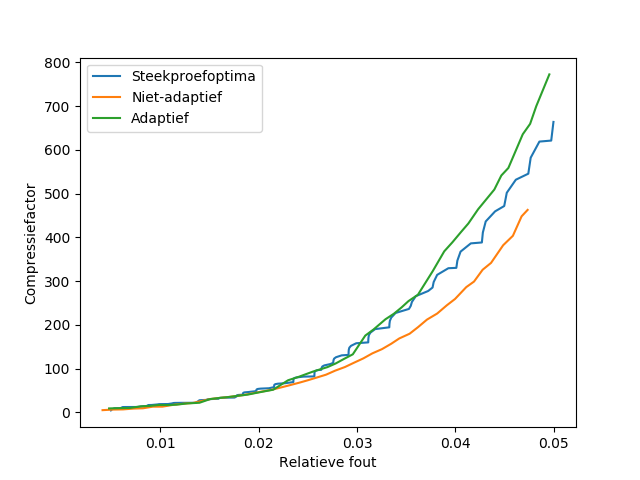
\includegraphics[scale=0.7]{images/parameter_functions_results_including_adaptive_Indian_Pines.png}
  \caption{Resultaten van compressie met adaptieve parameterselectie voor Indian Pines.}
  \label{fig:parameter_functions_results_including_adaptive_Indian_Pines}
\end{figure}

\newpage
\begin{figure}[H]
  \centering
  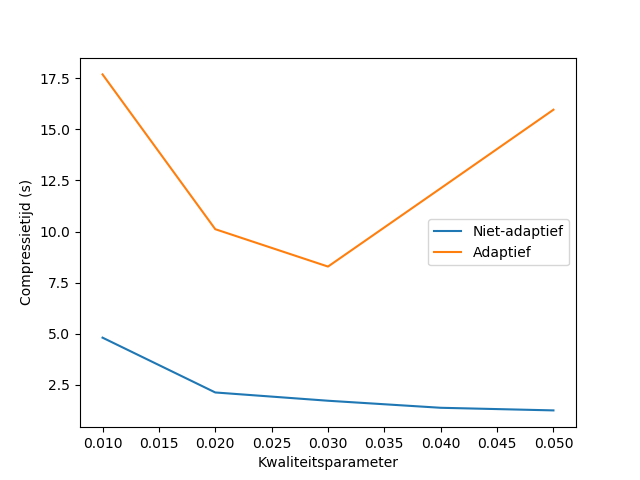
\includegraphics[scale=0.7]{images/adaptive_timings_Cuprite.png}
  \caption{Gemiddelde compressietijden voor verschillende kwaliteitsparameters voor Cuprite (10 experimenten).}
  \label{fig:adaptive_timings_Cuprite}
\end{figure}

\begin{figure}[H]
  \centering
  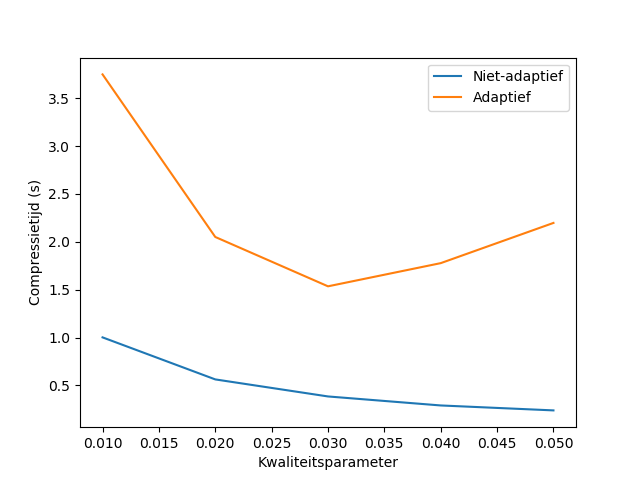
\includegraphics[scale=0.7]{images/adaptive_timings_Indian_Pines.png}
  \caption{Gemiddelde compressietijden voor verschillende kwaliteitsparameters voor Indian Pines (10 experimenten).}
  \label{fig:adaptive_timings_Indian_Pines}
\end{figure}
